%--------------------
% Packages
% -------------------
\documentclass[11pt,a4paper]{article}
\usepackage[utf8x]{inputenc}
%\usepackage{gentium}

\usepackage[pdftex]{graphicx} % Required for including pictures
\usepackage[pdftex,linkcolor=black,pdfborder={0 0 0}]{hyperref} % Format links for pdf
\usepackage{calc} % To reset the counter in the document after title page
\usepackage[english]{babel}     % for proper word breaking at line ends
\usepackage{graphicx}           % for ?
\usepackage{amsmath,amssymb}    % for better equations
\usepackage{amsthm}             % for better theorem styles
\usepackage{mathtools}          % for greek math symbol formatting
\usepackage{varwidth}
\usepackage{enumitem}           % for control of 'enumerate' numbering
\usepackage{listings}           % for control of 'itemize' spacing
 \setlength {\marginparwidth }{2cm}
\usepackage{todonotes}          % for clear TODO notes
\usepackage{pgfplots}
\usepackage{caption}
\usepackage{parskip}
\usepackage{makecell}
\usepackage{tabularx} 

\usepackage[a4paper, lmargin=0.1666\paperwidth, rmargin=0.1666\paperwidth, tmargin=0.1111\paperheight, bmargin=0.1111\paperheight]{geometry} %margins
%\usepackage{parskip}

\usepackage[all]{nowidow} % Tries to remove widows
\usepackage[protrusion=true,expansion=true,stretch=10]{microtype} % Improves typography, load after fontpackage is selected
\usepackage{hyperref}

\title{Research proposal master thesis: \\ Authenticated video conferencing in PubHubs}
\author{Julian van der Horst}

%-----------------------
% Begin document
%-----------------------
\begin{document} 
\maketitle
\section{Introduction}
In this thesis, we will do research into authenticated video conferencing in PubHubs. The research will be about the challenges and architectural designs needed to make such a feature, particularly looking into the security and privacy aspects of such a system and keeping them in line with the security and privacy considerations already made in PubHubs. We will propose a video conferencing architecture and build a prototype. In the thesis we will discuss the different options, choices and compromises made, limitations and dependencies. 

This research will also include a section on discussing the current landscape of authenticated video conferencing. We will consider alternatives and look at the importance of authenticated video conferencing following recent events.

\section{PubHubs}
Let us start by introducing PubHubs. PubHubs, short for Public Hubs, is an alternative community platform that puts public values first \cite{PH}. Unlike mainstream social media platforms like Instagram or Twitter that focus on individual broadcasting, PubHubs emulates real-world social dynamics by centering interactions within smaller, community-based hubs. The reasoning behind that is that this behavior closely resembles normal human interaction, where humans have small groups of friends and collaborators with whom they interact. The way people experience social media now is very unnatural, where if they engage with a platform, their posts are shouted into the whole world and are for everyone to see.

“PubHubs is organized as a network of independent hubs, with a shared single-sign-on. Conversations take place in local hubs (and not globally) and the associated (conversation) data is managed decentrally, within each hub” \cite{PH}. Privacy is one of the core values of PubHubs, which can be seen in how it handles identity management. The main idea of Pubhubs is to allow pseudonymity while maintaining both accountability and the ability to verify certain attributes of the user. The authentication of users is done using Yivi (formerly IRMA)\cite{YIVI} and the identity (the pseudonym) is generated using PEP \cite{PEP}. In PubHubs all communication is done via Matrix. “Matrix is an open-source network for secure, decentralized communication” \cite{MATRIX}.

\section{Video conferencing}
During the COVID-19 pandemic, there was a big need for remote work. Immediately, services like Zoom \cite{Zoom}  and Microsoft Teams  \cite{MSTeams} gained widespread adoption. These tools allowed video conferencing between different remote locations in real-time. These video call services might include end-to-end encryption but often lack authenticated video conferencing. Perhaps the need for authenticated video conferencing is not very apparent, and when calling friends it might not be needed. In contrast, when having an online consultation with your doctor, you want to be sure that you are actually calling a doctor.

If we look at video conferencing from a conceptual perspective, we see that there are multiple conferencing setups. For this research, we will distinguish three types. Person-to-person (one-on-one), Person-to-person (multiple people), and speaker-to-audience. We distinguish these types because they all have certain properties that best match with different technologies. Where in one-on-one we only need to send and receive to one other person, when we are in a group we need to send and receive data to each member in a call. On the contrary, with speaker-to-audience, we do not have connections between the individual audience members. The first and second setup are more in line with what we expect the users of Pubhubs to use video conferencing for, so we will focus on them in this research. 

\begin{figure}[!hbt]
    \centering
    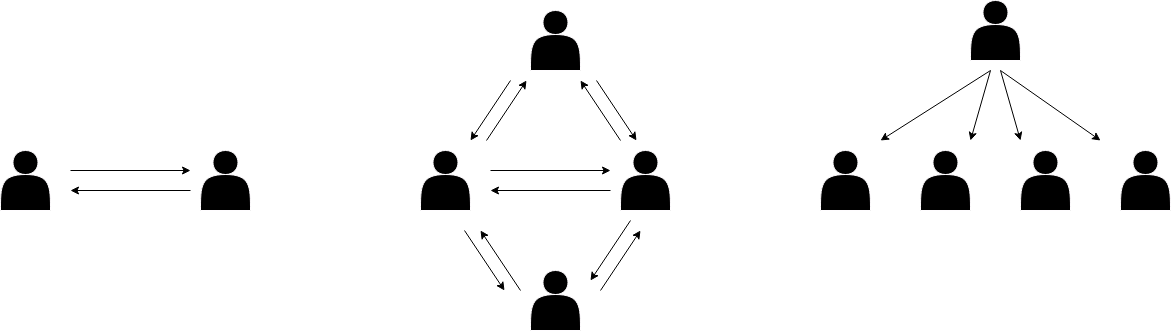
\includegraphics[width=0.7\textwidth]{Research proposal/img/three types.drawio.png}
    \caption{The three types of video conferencing}
    \label{fig:enter-label}
\end{figure}

With video conferencing, people need to send and receive video streams, and we want to do this ideally in real time. A standard for that is WebRTC, and it is now widely supported in browsers (97.77\%) \cite{CIUIWEBRTC}. WebRTC is both a protocol and an API that can be used for many things, including video and audio communication. Matrix even has support for WebRTC and uses it in their main testing application Element \cite{ELEMENT}. In our implementation, we will use WebRTC to send video and audio streams. However, to which endpoints do we need to send these WebRTC streams?

The first option is to send the data in a Peer-to-peer (P2P) network. This means that the people in the call send their stream to every other person in the call. This ensures that the server has no extra load since it does not handle any video streams, it simply facilitates the call setup. However, with every extra participant, every user needs to send/receive more and more data. At some point, a bottleneck is reached, and no extra participant can be added or a loss in data will occur. This is a very privacy-friendly method since the server has no access to the video conferencing data being sent and the users have full autonomy to choose who can receive their video data. However, due to the limited number of participants, this solution is not feasible.

Another option would be to have a Multipoint Control Unit (MCU). An MCU takes in many media streams and combines them into one media stream. This makes it so that it can work very well with legacy systems, since an MCU can receive various types of media and then output a standardized output. For example, this would allow a participant to call in from a phone connection while the other participant have a video call. The MCU has to decode all the incoming media signals, which makes it costly at large scale, since the CPU usage would be very high. From a security and privacy perspective, this solution is not ideal, since the server has access to all the unencrypted video and audio data. 

Lastly, we have the Selective Forwarding Unit (SFU). An SFU behaves in a way like a switch where it would selectively forward streams between clients, it does not interact with the video streams so it would work similarly with encrypted and unencrypted data. From a user perspective, we only need to talk to one server, and we send and receive all our data through that server. An SFU provides a compelling balance of scalability and privacy. it needs lower resources since it only needs to forward the signals to the users and does not decrypt the data. 

\section{Matrix and Element call}
As mentioned previously, Pubhubs uses Matrix when sending messages. Matrix not only used in sending messages and multimedia between users, but it is fundamentally used to create and manage the rooms in Pubhubs. Thus, when creating the architecture and prototype, the matrix protocol should be considered as to not make choices which directly oppose the matrix standard. The community can suggest changes to the Matrix protocol by submitting proposals, and over the years this has added a lot of functionality to Matrix. In proposal 3401 \cite{MATRIX_VIDEO_CALL_PROP}, functionality for video conferencing was proposed. This proposal can be applied to all the above-mentioned server setups and describes a protocol for video conferencing. 

The same team that built matrix is also building Element \cite{ELEMENT}, which is an open-source implementation of a messaging app that uses matrix. A new feature was added to Element called Element call, which serves as an example implementation of the proposal mentioned above. They started by using peer-to-peer video conferencing, since this more closely resembled the decentralized infrastructure of Matrix. However, this turned out to not be the best solution since it allowed for a maximum of 7 participants and video conferencing required numerous computer resources from participants. Recently, they have released a new version that makes use of an open-source SFU called Livekit \cite{LIVEKIT}.

We will use this implementation as a guide during our research; however, we will evaluate all the different choices made for Element call and deviate from them based on the requirements of PubHubs. When using Livekit we can easily implement features like noise suppression or video simulcast (Sending multiple video streams with different qualities, to dynamically choose the quality according to a user's internet connection).

\newpage
\section{Research question}
The main research question will be \textbf{“How can we design and implement an authenticated video conferencing solution within PubHubs that balances privacy, security, and usability?”}. This main question creates several sub-questions. We will divide these up into three different categories.

\textbf{Privacy}
For Pubhubs privacy is one of their core values and during the creation and development of Pubhubs certain decisions have been made regarding privacy. These decision should be considered and can be formulated into these sub-questions:

— What information or metadata should we allow leaking to achieve authenticated video conferencing, regarding the current Pubhubs privacy principles?

— How can we balance essential call features, like visible call status, with a commitment to user privacy?

\textbf{Encryption}
One of the foremost considerations in GDPR compliance for video conferencing is the implementation of end-to-end data encryption. This requires an encryption scheme which is user-friendly, has low computational overhead, and still has appropriate security.

— What encryption scheme is best suited for authenticated video conferencing in Pubhubs, weighing user experience and computational overhead while ensuring optimal security? 

\textbf{Development}
While doing the research and writing the code for it, we should also keep in mind the current development setup for PubHubs. This means that we should keep in mind which technologies they are using now and remain in those ecosystems. This makes it so that the code can be more easily maintained in the future. Pubhubs allows hubs to create their own version of the hub client, which should be considered when creating the video conferencing client.

— How can we develop a video conferencing prototype within the existing Pubhubs ecosystem, while simultaneously considering different hub client implementations?

\textbf{Societal Importance}
we will also discuss authenticated video conferencing from a bigger perspective. Some recent events have shown the importance of authenticated video calls. Like the German army official's video call incident \cite{GERMAN} and recently with generating AI videos becoming a trivial task \cite{SORA}\cite{HEYGEN}, it is important to know who you are talking to. Authenticated video conferencing is particularly important for certain sectors and institutions, such as healthcare. 

— Why hasn't authenticated video conferencing become mainstream, especially in institutions needing secure communications?

\bibliographystyle{plain}
\bibliography{main.bib}

\end{document}
